\documentclass[12pt, a4paper]{report} \usepackage[titletoc]{appendix}
%\linespread{1.5}
%\usepackage{lineno}
%\linenumbers
\usepackage{appendix}
\usepackage{multirow}
\usepackage{hhline}
\usepackage{array}
\usepackage{caption}
\usepackage{subcaption}
\usepackage{float}
\usepackage{graphicx}
	\graphicspath{{images/}} 
\usepackage{geometry}
	\geometry{a4paper,left=3cm,top=3cm,bottom=3cm,right=3cm}
\usepackage{array}
\usepackage{multirow}
\usepackage{hyperref}
	\hypersetup{colorlinks=true,allcolors=blue}
\usepackage{hypcap}
\usepackage[linesnumbered,ruled]{algorithm2e}
\usepackage{courier}
\usepackage{listings}
\lstset{
	basicstyle=\ttfamily,
	frame=none, 
	breaklines=true,
	numbers=left,
	xleftmargin=2.5em,
	framexleftmargin=0em,
	emphstyle=\textbf,
	float=t
}
\lstdefinestyle{ocl}{
	emph={
		context, inv
	}
}
\lstdefinestyle{change-based persistence}{
	basicstyle=\ttfamily\scriptsize,
	emph={
		session, create, of, type,
		set, to, add, hire
	}
}
\lstdefinestyle{xmi}{
	basicstyle=\ttfamily\scriptsize,
	emph={
		Node, children,
		Employee, manages
	}
}
\lstdefinestyle{xml}{
	basicstyle=\ttfamily\scriptsize,
	emph={
		register, create, add, to, resource,
		from, eattribute, remove, ereference,
		set, unset, session, Roy, Jen,
		Moss, Richmond
	}
}
\lstdefinestyle{java}{
	basicstyle=\ttfamily\scriptsize,
	emph={
		case, UNSET,
		instanceof, else, if, void,
		new, UnsetEAttributeEvent,
		UnsetEReferenceEvent,
		@override, public, class, extends
	}
}
\lstdefinestyle{eol}{
	basicstyle=\ttfamily\scriptsize,
	emph={
		var, new, for, in, create, set, of, with, 
		unset, to, add, remove, delete, register,
		from, position, from, move-within, session, \.
	}
}

\setlength{\parindent}{1cm}
\setlength{\parskip}{0.1cm}


\begin{document}

\begin{titlepage}
 \begin{center}

\textbf{Progress Report}
\vspace{1cm}

\textbf{\large Model Change-Based Persistence}
\vspace{1cm}

Alfa Ryano Yohannis\\
ary506@york.ac.uk
\vspace{1cm}

Supervisors:\\
Dimitris Kolovos\\
Fiona Polack\\
\vspace{1cm}

Department of Computer Science\\
University of York\\
United Kingdom\\
\vspace{1cm}
\today
 
\vfill
 
\end{center}
\end{titlepage}


\begin{abstract}
\addcontentsline{toc}{chapter}{Abstract}
Most of the models in Model-Driven Engineering are persisted in state-based formats. As an alternative, change-based persistence (change-based persistence) also has been proposed. State-based persistence (state-based persistence) offers faster model loading time than change-based representation but outperformed by its counterpart when it comes to persisting and detecting changes of models. This research aims to integrate both types of persistence to produce a hybrid model persistence to gain the advantages of both approaches. The main impact of change-based persistence on faster persisting and detecting changes, its knock-on effects on the model comparison and merging, as well as efforts to reduce its side effects will be investigated and evaluated. So far, an initial implementation has been developed, and an algorithm to reduce the loading time of change-based models has been proposed. Based on this work's previous investigation, change-based approach persists changes of models faster than its state-based counterpart, and the proposed algorithm has successfully loaded change-based models faster than loading the models naively. The initial implementation has been presented in a workshop, and the proposed algorithm has been submitted to a conference and currently under review. A research plan to complete this work in the next two years is also explained in this report.
\end{abstract}

\tableofcontents
\addcontentsline{toc}{chapter}{Contents}

\listoffigures
\newpage
 
\listoftables
\newpage

\lstlistoflistings
\newpage

\chapter{Introduction}
\label{ch:introduction}
This Chapter briefly presents the background of this work as well as the research questions that will address in this work. Several research objectives are then defined to answer the research questions. Research outputs and scoping are also presented. 

\section{Background}
\label{sec:background}
Most of models in the context of Model-Driven Engineering are persisted in state-based formats. In such approaches, model files contain snapshots of the models' contents, and activities like version control and change detection are left to external systems such as file-based version-control systems and model differencing facilities. Activities such as change-detection -- identifying parts that already changed of a model compared to its previous version/ancestor -- and model comparison -- finding the differences between models that come from the same ancestor -- are computationally consuming for state-based models. As a result, the expensive cost can become a burden for managing large models (e.g. identifying elements of a large model that have changed to execute certain model transformations) and when large models are developed in a collaborative setting (e.g. large models are developed in parallel and at some time  need to be compared and merged).

As an alternative to state-based persistence, this work proposes that a model can also be persisted in state-based format that is persisting the full sequence of \emph{changes} made to the model. The concept of change-based persistence is not new and has been used in persisting changes in software, object-oriented databases, and documents \cite{mens2002state,DBLP:conf/sde/LippeO92,DBLP:conf/caise/IgnatN05} and they reported that the approach can improve detecting differences more precisely at the semantic level -- that is by providing finer-granularity information (e.g. types of changes, the order of the changes, elements that were changed, previous values, etc.) -- and therefore provide supports to resolve them. The ordered nature of change-based persistence means that changes made to a model can be identified sequentially without having to explore and compare all elements of the model and its previous version. Based on these arguments, this work proposes change-based persistence as an alternative approach to state-based persistence to persist models. Persisting models in change-based format will bring a number of envisioned benefits over state-based persistence, such as the ability to detect changes much faster and more precise, which can then have positive knock-on effects on helping developers compare and merge models in collaborative modelling environments. 

Nevertheless, change-based persistence also comes at the cost of larger and ever-growing model files, and increased model loading time. A model that is modified frequently will increase considerably in file size since every change is added to the file. The increasing file size (proportional to the number of persisted changes) will increase the loading time of the model since all changes have to be replayed to reconstruct the model's eventual state. This downsides have to be mitigated to optimise the adoption of change-based persistence. One approach to reduce a change-based model's file size is by removing changes that do not effect the eventual state of the model. For the increased loading time, it can be mitigated by ignoring -- not replaying -- changes that are cancelled out by preceding changes or employing change-based and state-based persistence side-by-side so that the benefit of state-based persistence on loading time can still be obtained.   

%The expensive cost of state-based models in change-detection and model differencing motivates this work to investigate change-based persistence to enable fast model comparison and differencing, and scales for large models developed in a collaborative setting. So far, this research had already attempted to reduce the loading time of change-based persistence (change-based persistence) models and can save up 44\% loading time compared to loading change-based models naively (see Subsection \ref{sec:load_time_reduction_of_change-based_models} and Chapter \ref{ch:research_plan}, Task 1). However, since the optimised loading time is still significantly longer than the loading time of state-based persistence (state-based persistence), this research proposes a hybrid model persistence (hybrid persistence) that is persistence using change-based and state-based approaches side-by-side. Every event of model modification is persisted into a change-based representation, and the change is applied to a state-based representation simultaneously. This dual persistence enables faster change-detection while still maintains the loading time of state-based persistence and its other advantages as well, such as partial and lazy loading of model elements \cite{ran2016partial,daniel2016neoemf}.  

\section{Research Questions}
\label{sec:research_questions}
This work proposes a hypothesis, \textbf{``Change-based persistence reduces the execution time of model change-detection, model comparison, and model merging for large models compared to their execution time in state-based persistence, with relatively acceptable trade-off on model load time, persisting changes, memory footprints, and disk space consumption''}. The execution time is the time required to complete the processes (e.g. change-detection, model comparison, model merging, or persisting changes). Model change-detection is identifying changed elements of a model compared to its previous version/ancestor. Model comparison is finding the differences of two models that come from the same ancestor. Model merging is resolving conflicts two models that come from the same ancestor and merge them to produce a new model. The conflicts are resolved by predefined rules since it is unlikely to involve human to resolve large conflicts in large models. Large models preferably are models that consist of more than 1,500,000 elements as has been experimented in \cite{daniel2016neoemf,pagan2011morsa}. Model load time are the amount of time required to load a model into memory. Persisting changes is saving changes made to a model into a persistence representation (e.g. a file). For state-based models, this requires saving the entire model, except for state-based persistence that supports partial queries. Memory footprints are the sizes of memory used to execute the processes. Disk space consumption is the amount of space in storage consumed by the persistence.  

Thus, in order to confirm the hypothesis, this work aims to answer these following research questions: 
\begin{enumerate} 
	\item \textbf{How to persist changes in change-based format? How does it perform compared to state-based persistence on saving changes?} 
	
	The concept of change-based persistence has to be translated into an implementation in a modelling framework context so that it can be applied for model persistence, and therefore its impact on model change-detection, model comparison, and model merging can be assessed. It is expected that every change made to a model can be persisted by the implementation and can reconstruct the same model persisted in state-based format after replaying all the changes. It is also expected that change-based persistence will outperform state-based persistence on the time required for saving changes since change-based persistence will only requires to persist changes of a model while state-based persistence will persist the whole model. 
	
	\item \textbf{How to reduce the increasing file size and loading time of change-based models? And to what extent can they be reduced?} 
	
	Change-based persistence comes with downsides on larger, increasing file size and loading time. Mitigating these side effects will optimise the use of change-based persistence. For the increasing file size, the size can be reduced by removing changes that do not effect the eventual state of the model. For the increasing loading time, it can be mitigated by ignoring -- not replaying -- changes that are cancelled out by preceding changes or employing change-based and state-based persistence side-by-side so that the benefit of state-based persistence on loading time can still be obtained. It is expected that: (1) the mitigation approaches will produce loading time that is closer to the loading time of state-based format, (2) the mitigation approaches will significantly load models faster than loading change-based models naively, and (3) the mitigation approaches will significantly reduce change-based model file sizes compared to the naive approach on saving change-based model files. 

	For reducing the loading time using change-based and state-based persistence side-by-side, th impact of the approach will also be investigated on several qualities. It is expected that: (1) hybrid persistence approach will be significantly slower than change-based persistence on persisting changes and slightly slower than state-based persistence on saving time as the hybrid approach will need to save changes to the other two types of persistence. (2) The hybrid approach will consume more disk space compared to change-based or state-based persistence since the hybrid approach will use them both simultaneously. (3) The hybrid approach will have loading time that is closer to the loading time of state-based persistence. 
    
    \item \textbf{How to detect changes in change-based models -- comparing them to their ancestors/previous versions? And to what extent does the change-detection of change-based models perform compared to change-detection in state-based models?} 
        
    The purpose of using change-based persistence in this work is to improve change-detection. The change-based persistence will have change-detection time that is smaller than the change-detection time of state-based persistence.        
	
	\item \textbf{How to compare change-based models that come from the same ancestor? And how does the comparison of change-based models perform compared to the state-based model comparison?} 
	
	The knock-on effect of faster change-detection on model comparison will also be investigated. Due to the nature of change-based models, the mechanism to perform change-based model comparison will differ substantially from the current state-based model comparison. It is expected that comparison of change-based models will be significantly faster than the comparison of state-based models.   
	
	\item \textbf{How to merge different change-based models that come from the same ancestor? And how does the merging perform compared to model merging in state-based persistence?}
	
	Another knock-on effect of faster change-detection of change-based persistence is faster model merging. Similar to change-based model comparison, the mechanism to merge change-based models will differ substantially from merging state-based models. It is expected that the change-based model merging will be much faster than state-based model merging.   
	
\end{enumerate}

\section{Research Objectives}
\label{sec:research_objectives}
This research aims to meet the following research objectives to answer the research questions.
\begin{enumerate}
	\item Develop an implementation of change-based persistence so it can be applied to persist models in change-based format, and evaluate the correctness of change-based models that it produces and its performance on saving changes against state-based persistence. 
	\item Propose approaches to reduce the increasing file size and loading time of change-based persistence models, and evaluate their performance against naive approaches. For the increasing file size, it will be reduced by removing changes that do not effect the eventual state of the model. For the increasing loading time, it will be reduced by ignoring -- not replaying -- changes that are cancelled out by preceding changes or employing change-based and state-based persistence side-by-side so that the benefit of state-based persistence on loading time can still be obtained.    
    \item Develop a solution to detect changes in change-based models, and evaluate its execution time and memory footprint against change-detection in state-based models.
	\item Develop a solution to compare change-based models, and evaluate its execution time and memory footprint against model comparison in state-based models.
	\item Develop a solution to merge different change-based models, and evaluate its execution time and memory footprints against model-merging in state-based models. 
\end{enumerate}

\section{Research Outputs}
\label{sec:research_outputs}
By the end of this research, these following outputs will have been produced:
\begin{enumerate}
	\item Prototypes for change-based persistence and hybrid model persistence so they can be implemented to persist models. 
	\item Solutions -- including their implementation and evaluation -- for file size and loading time reduction, change-detection (finding parts that already changed of a model compared to its previous version/ancestor), model comparison (finding differences between models that come from the same ancestor), and model merging of change-based persistence.
	\item A publication for each research question, and a thesis report of this research. 
\end{enumerate}


\section{Research Scope}
\label{sec:research_scope}
Since this research will also use change-based and state-based persistence side-by-side, an existing instance of state-based persistence is required for executing the implementation and evaluation. NeoEMF \cite{daniel2016neoemf}, a recent work that leverages the use of NoSQL databases for large-scale model persistence, is considered for this research. 

All technical implementations or prototypes in this research will be developed in the context Eclipse Modelling Framework. Other similar modelling frameworks are not parts of this research scope. 


\chapter{Progress Review}
\label{ch:progress_review}
This chapter presents the progress of this research. It comprises literature review and the results of Task 1 (Chapter \ref{ch:research_plan}) that have been presented in a workshop and submitted in a conference (Chapter \ref{ch:publications}). 

\section{Research Methodology}
\label{sec:research_methodology}
This research is using the Design Science Research Methodology (DSRM) \cite{peffers2007design} as its research methodology. DSRM is a methodology intended to guide the production and presentation of Design Science research in Information Systems. Design Science itself is essentially a problem-solving paradigm through the applications of artefacts which must be designed, built, and evaluated \cite{hevner2010design}. The artefacts can be constructs (vocabulary and symbols), models (abstractions and representations), methods (algorithms and practices), and instantiations (implemented and prototype systems) \cite{hevner2004design}. Although originally intended for Information Systems, the same approach can also be applied in Model-Driven Engineering since both address problems through the creation of technological artefacts. DSRM consists of six activities: identify problem and motivation, define objectives for a solution, design and development, demonstration, evaluation, and communication. These six activities are set at the high level of abstraction therefore it allows users to select context-specific methods to be executed in each activity. The specific methods for each of the six activities are as follows and summarised in Table \ref{table:research_progress}.

\begin{enumerate}
    \item \textbf{Identify Problem and Motivation}. Research should define the specific research problems and justify the value of a solution. This work will conduct literature review and exploring existing tools that are relevant to this research to identify the problems and the motivation.
    \item \textbf{Define Objective for a Solution}. Research should infer the objectives of a solution from the problem definition and knowledge of what is possible and feasible. The solution and its objectives will be derived from the problems and motivation defined in the previous activity, and from the knowledge gained from the literature review and existing tool exploration.
    \item \textbf{Design and Development}. Artefacts should be designed and developed. This activity includes determining their functionalities, architectures, or underlying knowledge to create the artefacts to bring in solutions. This research will follow the best practices of software development, such iterative and incremental design and development, unit testing, and version control.
    \item \textbf{Demonstration}. Artefacts should demonstrate how they solve the problems. The solution developed in this research will be demonstrated in simulation and experimentation. 
    \item \textbf{Evaluation}. Artefacts should be measured how well they solve the problems. Empirical comparative study will be used as the method to measure the qualities of the proposed solution compared to baselines -- relevant existing approaches or conditions that the solution seek to improve.
    \item \textbf{Communication}. The research of design artefacts has to be disseminated. This work will be communicated through academic reports, journals, workshops, and conferences.
\end{enumerate}

\begin{table}[h]
    \centering
    \caption{DSRM's activities and their methods and current results of this research.}
    \label{table:research_progress}
    \begin{tabular}
        {|>{\centering\arraybackslash}p{0.6cm}|>{\centering\arraybackslash}p{3cm}|>{\centering\arraybackslash}p{3.1cm}|>{\centering\arraybackslash}p{6.5cm}|}
        \hline 
        \textbf{No}&\textbf{Activities}&\textbf{Methods}&\textbf{Current Results}\\
        \hline 
        1 & Problem and Motivation &literature review, tool review & research background (Section \ref{sec:background})\\
        \hline 
        2 & Objectives & literature review, tool review & a hypothesis, research questions (Section \ref{sec:research_questions}) and objectives  (Section \ref{sec:research_objectives})\\
        \hline 
        3 & Design and Development & iterative and incremental approach, unit testing, version control & the division of this research into several tasks (Chapter \ref{ch:research_plan}), change-based persistence prototype, and loading optimisation algorithm for change-based models\\
        \hline 
        4 & Demonstration & simulation, experiments  & (1) the implementation of the change-based approach can save and load change-based models, and (2) the proposed loading optimisation algorithm can reduce the loading time of change-based models \\
        \hline 
        5 & Evaluation & empirical comparative study & (1) change-based approach persists changes of models faster than state-based approach, and (2) the proposed loading algorithm loads change-based models faster than naive loading approach but significantly produces more memory footprints and is still outperformed by state-based persistence\\
        \hline 
        6 & Communications & reports, journals, workshops, conferences & one workshop paper (presented) and one conference paper (under review)\\
        \hline 
\end{tabular} 
\end{table}
        

\section{Current Progress and Results}
\label{sec:current_progress_and_results}
This section summarises the work that have been done so far and shows how the methods mentioned previously contribute to this research. This section also summarises any results that have been obtained and outline their significance -- they contribution to the research questions or hypothesis. The current progress and results of this research is summarised in Table \ref{table:research_progress}.

\subsection{Identify Problem and Motivation}
\label{subsec:identify_problem_and_motivation}
This work has conducted a literature review and existing tool exploration to identify problem and motivation for research. The problem and motivation are presented in Section \ref{sec:background}.

\subsection{Define Objectives for a Solution}
\label{subsec:define_objectives_for_a_solution}
Based on the problems and motivations presented in Section \ref{sec:background} and knowledge gained from literature review and existing tool exploration, this work has derived a hypothesis, research questions and objectives which are presented in Section \ref{sec:research_questions} and Section \ref{sec:research_objectives}. 

\subsection{Design and Development}
\label{subsec:design_and_development}
This work has been using iterative and incremental design and development, unit testing, and version control practices to design and develop the prototype or implementations required for this research. To facilitate the incremental development, the work is divided into several tasks (Chapter \ref{ch:research_plan}). Every task will address specific research question, and every subsequent task, to certain degree, depends on the results generated in the previous task (e.g. the implementation of change-based persistence is developed first so that change-detection, model comparison and merging of change-based models can be build upon it). To reach certain qualities and functionalities, the implementations has being developed iteratively. Unit testing is used to identify whether such qualities and functionalities have been satisfied or the design and development still need more refinement. Version control are used to manage versions of the implementation, such as creating a branch for experimenting a new idea and return to an older version because the new idea causes does not work. Overall, through this design and development activity, this work has been able to produce an implementation to persist changes of a model into a change-based representation and an implementation of an algorithm to reduce the loading time of change-based models.

\subsection{Demonstration}
\label{subsec:demonstration}

\subsection{Evaluation}
\label{subsec:evaluation}

\subsection{Communication}
\label{subsec:communication}
Two papers have been written (Appendix \ref{ch:publications}). The first paper \cite{yohannis2017turning} has been presented in the FlexMDE 2017 workshop and the second one \cite{yohannis2018algorithm} has been submitted to FASE 2018 conference and currently under review.

%%\section{Literature Review}
%%\label{sec:literature_review}
%%So far, review of the related literature has focused on model persistence and change detection. More literature review needs to be conducted on model comparison and merging.  
%%
%%\subsection{Change Detection}
%%\label{subsec:change_detection}
%%There are two approaches in the literature for identifying changes in models.
%%
%%\textbf{Notifications}. In this approach, changes of a model can be identified using  notification facility provided by a modelling tool. When a model is modified, the facility produces notification that carries information about the changes that had just occurred. This is an approach taken by the IncQuery incremental pattern matching framework \cite{rath2012derived} and the ReactiveATL incremental model-to-model transformation engine \cite{ogunyomi2015property}. The main advantage of this approach is that precise and fine-grained change notifications are provided for free by the modelling tool (and thus do not need to be computed, which as discussed below can be expensive and inefficient). On the downside, this approach is a poor fit for collaborative development settings where modelling and automated model processing activities are performed by different members of the team.
%%
%%\textbf{Model Differencing}. Instead of depending on live notifications, changes can be identified by comparing a model to its previous version using a model-differencing framework such as SiDiff \cite{kelter2005generic} or EMFCompare\footnote{\url{https://www.eclipse.org/emf/compare/}}. The main advantage of this approach is that it works well in a collaborative development environment where typically developers have distinct roles and responsibilities. On the downside, model comparison and differencing are computationally expensive and memory-greedy (both versions of the model need to be loaded into memory before they can be compared).
%%
%%\subsection{Model Persistence}
%%\label{subsec:model_persistence}
%%Several works have investigated alternative -- but also state-based -- model persistence mechanisms to XMI, mainly by leveraging databases (both relational and NoSQL). For example, EMF Teneo\,\cite{eclipse2017teneo} persists EMF models in relational databases, while Morsa \cite{pagan2011morsa} and NeoEMF \cite{daniel2016neoemf} persist models in document and graph databases respectively. The main challenge with such approaches is version control. None of these approaches provides built-in support for versioning and models are eventually stored in binary files/folders which are known to be a poor fit for text-oriented version control systems like Git and SVN.
%%
%%Connected Data Objects (CDO) \cite{eclipse2017cdo}, provides support for database-backed model persistence as well as collaboration facilities, but its adoption necessitates the use of a separate version control system in the software development process (e.g. a Git repository for code and a CDO repository for models), which introduces well-recognised fragmentation and administration challenges \cite{barmpis2014evaluation}. Similar challenges are related to the adoption of other model-specific version control systems such as EMFStore\,\cite{koegel2010emfstore}.
%%
%%\section{Change-based Persistence}
%%\label{sec:change-based_persistence}
%%This section illustrates the concept of change-based persistence (change-based persistence) and its technical implementation. This work has been presented in a workshop (Chapter \ref{ch:publications}, number 1). 
%%
%%\subsection{Introduction to Change-based Persistence}
%%\label{subsec:introduction_to_change-based_persistence}
%%Figures \ref{fig:initial_chart_0} and \ref{fig:modified_chart} are two consecutive versions of a sample organisational chart model. 
%%
%%\begin{figure}[ht]
%%	\centering
%%	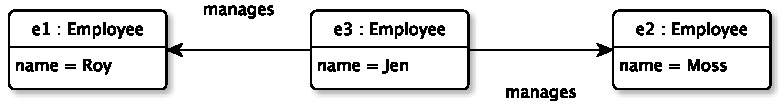
\includegraphics[width=\linewidth]{initial_chart_0}
%%	\caption{Initial version of the organisational chart model.}
%%	\label{fig:initial_chart_0}
%%\end{figure}
%%
%%\begin{figure}[ht]
%%	\centering
%%	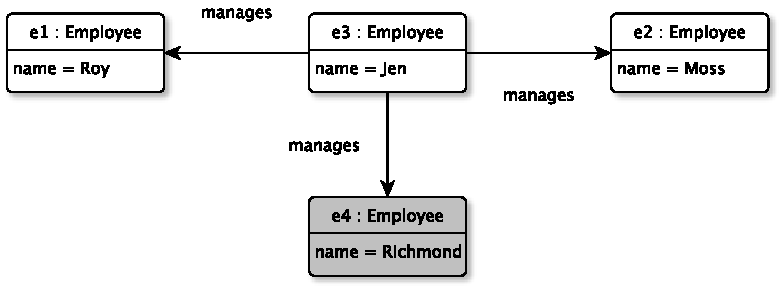
\includegraphics[width=\linewidth]{modified_chart}
%%	\caption{Modified version of the organisational chart model of Fig. \ref{fig:initial_chart}.}
%%	\label{fig:modified_chart}
%%\end{figure}
%%
%%To illustrate the proposed approach, List. \ref{lst:xmimodel_0} shows a state-based representation of the model of Fig. \ref{fig:modified_chart} in (simplified) XMI, and List. \ref{lst:change-based persistencemodel_0} shows the proposed equivalent change-based representation of the same model. Instead of a snapshot of the state of the model, the representation of List. \ref{lst:change-based persistencemodel_0} captures the complete sequence of change events (create/set/add/remove/delete) that were performed on the model since its creation, organised in editing sessions (2 editing sessions in the case of this model). Replaying these changes produces the same state as the one captured in List. \ref{lst:xmimodel}, so the proposed representation carries at least as much information as the state-based representation.
%%
%%\begin{lstlisting}[style=xmi,caption={State-based representation of the model of Figure \ref{fig:modified_chart} in (simplified) XMI.},label=lst:xmimodel_0]
%%<Employee xmi:id="e2" name="Jen">
%%<manages xmi:id="e1" name="Roy"/>
%%<manages xmi:id="e3" name="Moss"/>
%%<manages xmi:id="e4" name="Richmond"/>
%%</Employee>
%%\end{lstlisting}
%%
%%\begin{figure}[h]
%%	\begin{lstlisting}[style=xml,caption={Change-based representation of the model of Figure \ref{fig:modified_chart}.},label=lst:change-based persistencemodel_0]
%%	<session id="s1"/>
%%	<create eclass="Employee" epackage="employee" id="0"/>
%%	<add-to-resource position="0"><value eobject="0"/></add-to-resource>
%%	<set-eattribute name="name" target="0"><value literal="Roy"/></set-eattribute>
%%	<create eclass="Employee" epackage="employee" id="1"/>
%%	<add-to-resource position="1"><value eobject="1"/></add-to-resource>
%%	<set-eattribute name="name" target="1"><value literal="Jen"/></set-eattribute>
%%	<create eclass="Employee" epackage="employee" id="2"/>
%%	<add-to-resource position="2"><value eobject="2"/></add-to-resource>
%%	<set-eattribute name="name" target="1"><value literal="Moss"/></set-eattribute>
%%	<remove-from-resource><value eobject="0"/></remove-from-resource>
%%	<add-to-ereference name="manages" position="0" target="1"><value eobject="0"/></add-to-ereference>
%%	<remove-from-resource><value eobject="2"/></remove-from-resource>
%%	<add-to-ereference name="manages" position="1" target="1"><value eobject="2"/></add-to-ereference>
%%	<session id="s2"/>
%%	<create eclass="Employee" epackage="employee" id="3"/>
%%	<add-to-resource position="1"><value eobject="3"/></add-to-resource>
%%	<set-eattribute name="name" target="3"><value literal="Richmond"/></set-eattribute>
%%	<remove-from-resource><value eobject="3"/></remove-from-resource>
%%	<add-to-ereference name="manages" position="2" target="2"><value eobject="3"/></add-to-ereference>
%%	\end{lstlisting}
%%\end{figure}
%%
%%Such a representation is particularly suitable for change-detection. For example, if the model had been modified in the editing session \emph{s1}, further changes of the model can be readily identified since then (i.e. in session \emph{s2} –- lines 15-20) instead of having to rediscover them through (expensive) state-based model differencing.
%%
%%\subsection{Prototype Implementation of Change-Based Persistence}
%%\label{subsec:prototype_implementation_of_change-based_persistence}
%%This work has implemented a prototype\footnote{The prototype is available under \url{https://github.com/epsilonlabs/emf-change-based persistence}.} of the change-based model persistence format using the notification facilities provided by the Eclipse Modelling Framework. The implementation uses \emph{ChangeEventAdapter}, a subclass of EMF's \emph{EContentAdapter}, to receive and record \emph{Notification} events produced by the framework for every model-element level change.
%%
%%\begin{figure}[th]
%%	\centering
%%	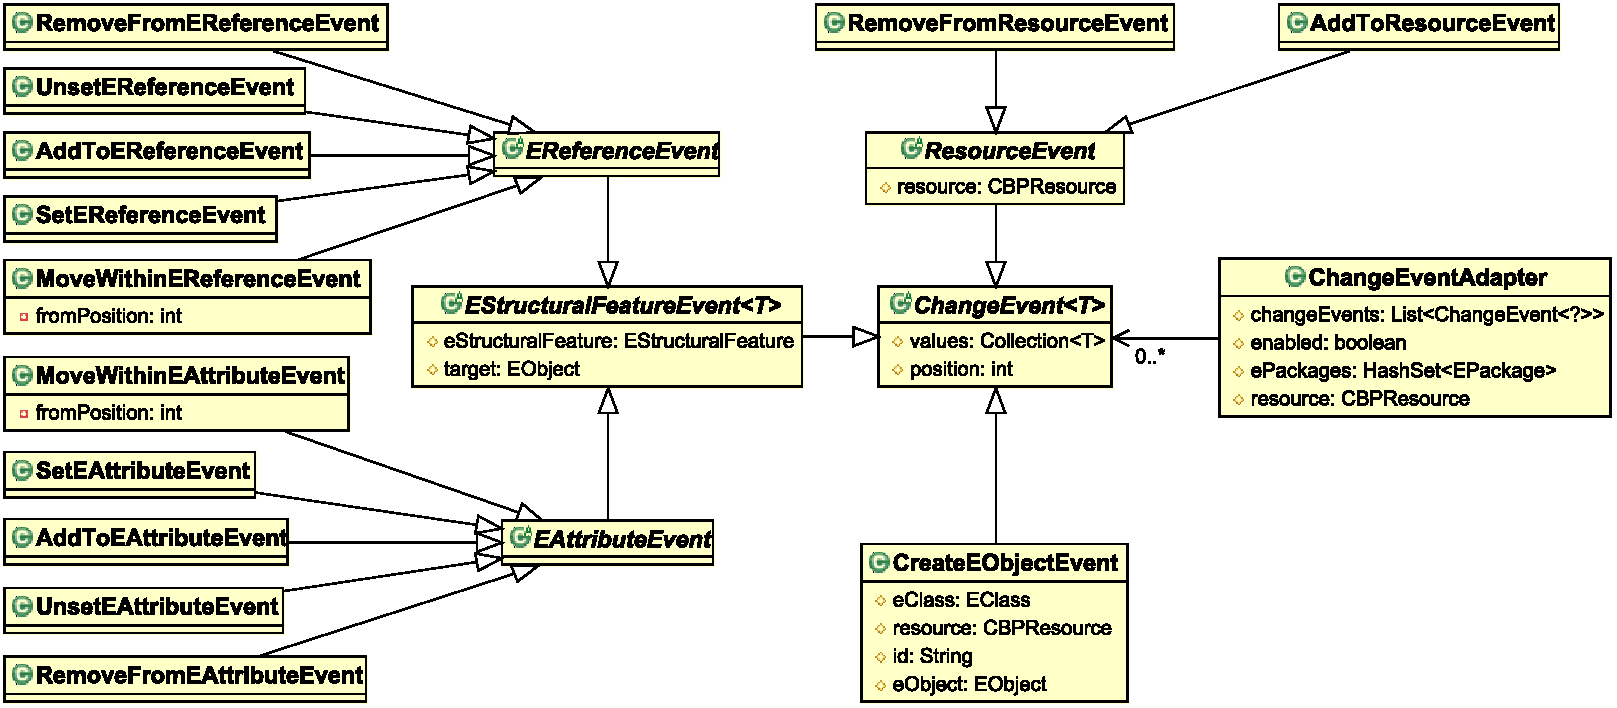
\includegraphics[width=\linewidth]{events}
%%	\caption{Event classes to represent changes of models.}
%%	\label{fig:events}
%%\end{figure}
%%
%%Since not all change events are relevant to change-based persistence (e.g. EMF also produces change notifications when listeners/adapted are added/removed from the model), this work has defined a set of event classes to represent events of interest. The event classes are depicted in Fig. \ref{fig:events} as subclasses of the \emph{ChangeEvent} abstract class. 
%%
%%The \emph{ChangeEvent} class has a multi-valued \emph{values} attribute which can accommodate both single-valued (e.g. set/add) or mutli-valued events (e.g. addAll/removeAll). \emph{ChangeEvent} can also accommodate different types of values, such as \emph{EObject}s for \emph{EReferenceEvents}, and primitive values (e.g. Integer, String) for \emph{EAttributeEvents}. The \emph{ChangeEvent} class also has a position attribute to hold the index of an \emph{EObject} or a literal when they are added to a \emph{Resource}, \emph{EReference}, or \emph{EAttribute} with multiple values (Lst. \ref{lst:change-based persistencemodel}, line 3, 6, 9, 12, 14, 17, 20). 
%%
%%Every time an \emph{EObject} is added to the model, a \emph{CreateEObjectEvent} and an \emph{AddToResourceEvent} are recorded (lines 2-3, 5-6, 8-9, and 16-17 in Lst. \ref{lst:change-based persistencemodel}). When an EObject is deleted or moved to a containment \emph{EReference} deeper in the model (Lst. \ref{lst:change-based persistencemodel}, line 12, 14, 20), a \emph{RemoveFromResourceEvent} (Lst. \ref{lst:change-based persistencemodel}, line 11, 13, 19) is recorded.
%%
%%\begin{lstlisting}[style=java,caption={Simplified Java code to handle notification events.},label=lst:javacode]
%%public class ChangeEventAdapter extends EContentAdapter {
%%...
%%@override
%%public void notifyChanged(Notification n) {
%%...
%%switch (n.getEventType()) {
%%... // other events
%%case Notification.UNSET: {
%%if (n.getNotifier() instanceof EObject) {
%%EStructuralFeature feature = (EStructuralFeature) n.getFeature();
%%if (feature instanceof EAttribute) {
%%event = new UnsetEAttributeEvent();
%%} else if (feature instanceof EReference) {
%%event = new UnsetEReferenceEvent();
%%}
%%} break;
%%} 
%%... // other events
%%\end{lstlisting}
%%
%%The \emph{ChangeEventAdapter} receives EMF change notifications in its \emph{notifyChanged()} method and filters and transforms them into appropriate change events. As an example of how notifications are filtered and transformed, Listing \ref{lst:javacode} shows how the implementation handles \emph{Notification.UNSET} events based on the type of the changed feature i.e. an \emph{UnsetEAttributeEvent} is instantiated if the feature of the notifier is an \emph{EAttribute}, or an \emph{UnsetEReferenceEvent} is created if the notifier is an \emph{EReference}. The transformed instances are then stored into a list of events in \emph{ChangeEventAdapter} (\emph{changeEvents}) for persistence. 
%%
%%\begin{figure}[th]
%%	\centering
%%	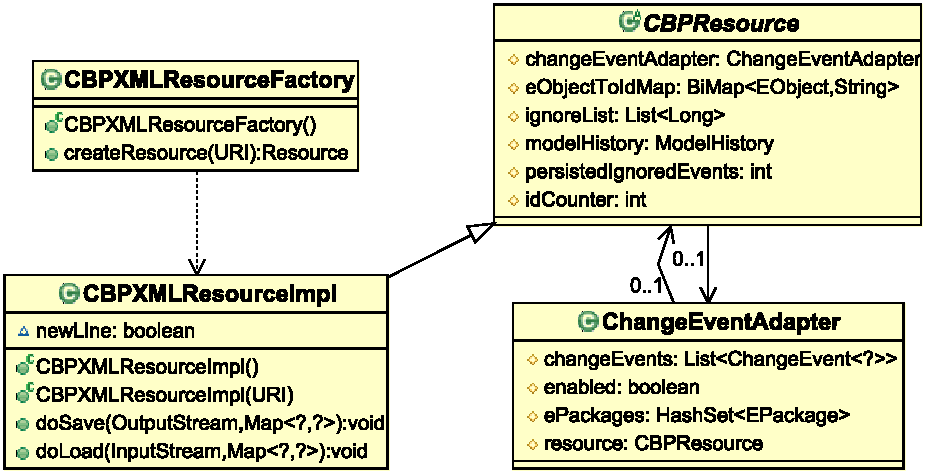
\includegraphics[width=0.6\linewidth]{resources}
%%	\caption{Factory, resources, and ChangeEventAdapter classes.}
%%	\label{fig:resources}
%%\end{figure}
%%
%%To integrate seamlessly with the EMF framework and to eventually support multiple concrete change-based serialisation formats (e.g. XML-formatted representation for readability and binary for performance/size), the implementation has created the \emph{change-based persistenceResource} abstract class, that extends EMF's built-in \emph{ResourceImpl} class. The role of the abstract class is to encapsulate all change recording functionality while the role of its concrete subclasses is to implement serialisation and de-serialisation. For example, \emph{change-based persistenceXMLResourceImpl} persists changes in a line-based format where every change is serialised as a single-line XML document. In this way, when a model changes, The implementation can append the new changes to the end of the model file without needing to serialise the entire model again. The implementation has also implemented a \emph{change-based persistenceXMLResourceFactory} class that extends EMF's \emph{ResourceFactoryImpl}, as the factory class for change-based models. Figure \ref{fig:resources} shows the relationships between these classes.
%%
%%\section{Load Time Reduction of Change-Based Models}
%%\label{sec:load_time_reduction_of_change-based_models}
%%This section re-illustrates the concept of change-based persistence (change-based persistence) for the purpose of explaining the algorithm used to reduce the loading time of change-based models. This work has been submitted to a conference (Chapter \ref{ch:publications}, number 2) and currently under review. 
%%
%%\subsection{Running Example}
%%\label{subsec:case_study}
%%To explain the change-based model persistence and the contribution of this work, the minimal tree metamodel is used (expressed in the Eclipse Modelling Framework's Ecore metamodelling language) and model illustrated in Figures \ref{fig:tree_metamodel} and \ref{fig:initial_model}. EMF/Ecore was selected as the de-facto standard for object-oriented metamodelling, and this contrived example to avoid unnecessary repetition in the discussion, while providing a reasonable coverage of the core features of Ecore (classes, single/multi-valued features, references and attributes). In this example, tree models consist of named nodes which can -- optionally -- contain other nodes (\emph{children} reference).
%%
%%\begin{figure}[ht]
%%	\begin{subfigure}[t]{0.4\linewidth}
%%		\centering
%%		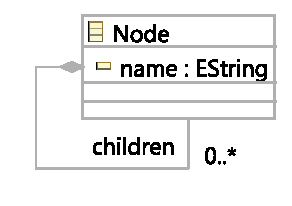
\includegraphics[width=0.8\linewidth]{node_metamodel}
%%		\caption{The tree metamodel.}
%%		\label{fig:tree_metamodel}
%%	\end{subfigure}
%%	\hfill
%%	\begin{subfigure}[t]{0.6\linewidth}
%%		\centering
%%		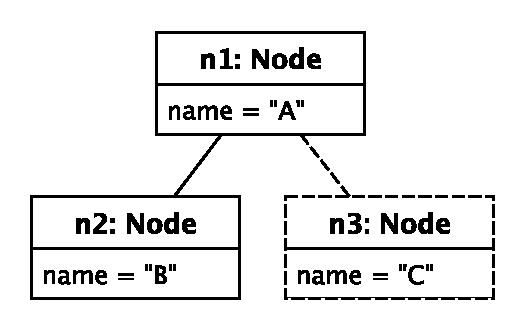
\includegraphics[width=0.6\linewidth]{initial_chart}
%%		\caption{A model that conforms to the tree metamodel (n3 was created and then deleted)}
%%		\label{fig:initial_model}
%%	\end{subfigure}
%%	\caption{A tree metamodel and its model as the running example.}
%%	\label{fig:append_speed}
%%\end{figure}
%%
%%\noindent
%%\begin{minipage}[t]{0.5\linewidth}
%%	\begin{lstlisting}[style=xmi,caption={State-based representation of the tree model in (simplified) XMI.},label=lst:xmimodel]
%%	<Node id="n1" name="A">
%%	<children id="n2" name="B"/>
%%	</Node>
%%	\end{lstlisting}
%%\end{minipage}
%%\hfill
%%\begin{minipage}[t]{0.5\linewidth}
%%	\begin{lstlisting}[style=eol,caption={Change-based representation of the tree model.},label=lst:change-based persistencemodel]
%%	create n1 of Node
%%	set n1.name to "A"      
%%	create n2 of Node
%%	set n2.name to "B"      
%%	create n3 of Node
%%	set n3.name to "C"      
%%	add n2 to n1.children   
%%	add n3 to n1.children
%%	remove n3 from n1.children   
%%	delete n3
%%	\end{lstlisting}
%%\end{minipage}
%%
%%The model in Fig. \ref{fig:initial_model} consists of two nodes \emph{n1}, \emph{n2}.
%%The construction of the model starts with creating and naming three nodes (\emph{n1}, \emph{n2} and \emph{n3}).
%%Nodes \emph{n2} and \emph{n3} were then added as children of \emph{n1}.
%%Finally, node \emph{n3} was deleted from the model.
%%The final state of the model is presented in a simplified (state-based) XMI representation in Listing \ref{lst:xmimodel}.
%%
%%In contrast to the state-based representation, a change-based persistence representation of the model is illustrated in Listing \ref{lst:change-based persistencemodel} (the syntax is a simplified version of the one introduced in\,\cite{yohannis2017turning}). Lines 1-6 record the creation and naming of the three nodes, lines 7 and 8 record the addition of \emph{n2} and \emph{n3} as children of \emph{n1} and lines 9-10 capture the deletion of \emph{n3} (deletion effectively involves a removal and a deletion event).
%%
%%For small changes made to large models, this approach can be beneficial since only the change events that need to be persisted every time -- as opposed to the entire model. However, loading the model by naively replaying all the events is not optimal particularly for models with long editing histories where prior events are often superseded by subsequent events. For example, creating \emph{n3} in line 5, naming it in line 6, and adding it to the children of \emph{n1} in line 8 are cancelled by the subsequent deletion of \emph{n3} in line 10. As such, the events in lines 5, 6, 8, 9 and 10 could be ignored during the loading process without affecting the eventual state of the model.
%%
%%The flowchart in Fig. \ref{fig:flowchart} provides an overview of the editing lifecycle of a change-based model, and the artefacts and data structures involved in it. It also highlights (starred blocks) the extensions proposed compared to the original change-based persistence approach in \cite{yohannis2017turning}.
%%
%%\begin{figure}[ht]
%%    \centering
%%    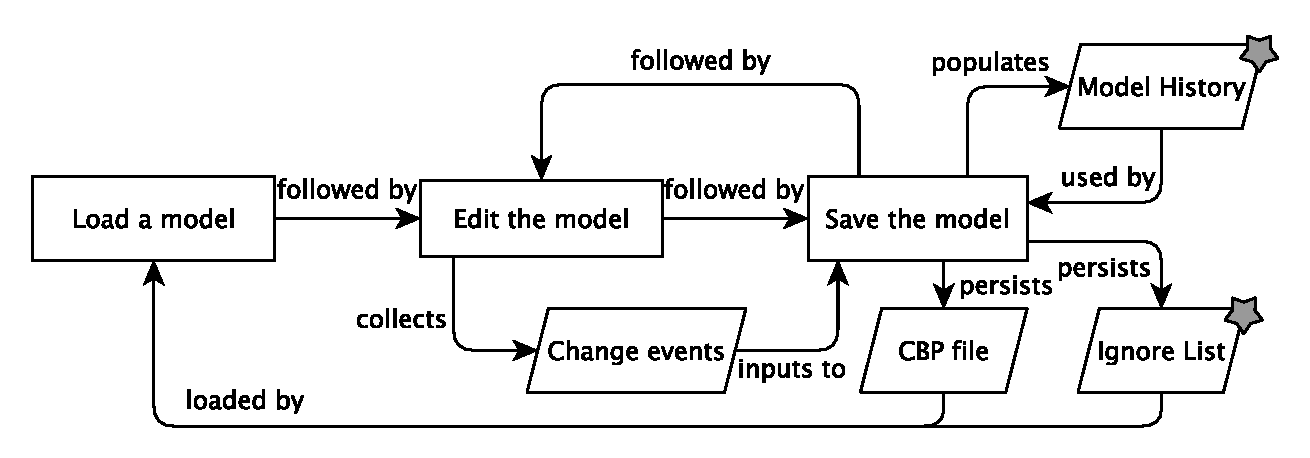
\includegraphics[width=\linewidth]{flowchart}
%%    \caption{The context flowchart of optimising loading performance of change-based persistence.}
%%    \label{fig:flowchart}
%%\end{figure}
%%
%%In the original change-based persistence approach, a model editing session involves three activities: loading a model, editing it, and saving new changes back to the model file\footnote{After saving a model, the user can make further changes and save it again.}. Loading is achieved by reading and replaying a sequence of change events stored in a change-based persistence-formatted file. During the editing process, changes to the model are stored in a memory-based data structure (``Change events''), which are serialised and appended at the end of the change-based persistence-formatted model file, and then flushed from memory, every time the model is saved.
%%
%%The proposed approach adds two new artefacts: a ``Model History'' data structure which is populated with change events and which is used to detect superseded events prior to saving, and an ``Ignore List'' file for each change-based model, which persists the position (i.e. line numbers) of superseded events so that they can be ignored the next time the model is loaded.
%%
%%\subsection{Model History}
%%\label{subsec:model_history}
%%The proposed approach uses a data structure that memorises elements' events and their position (line number) in a change-based persistence representation so it can reason about the events of a particular element and determine which of them are superseded. For the rest of the discussion, the line number in the change-based persistence representation is referred to as the \emph{event number}. The proposed data structure is presented in Fig. \ref{fig:object_history} as a class diagram.  
%%
%%\begin{figure}[ht]
%%	\centering
%%	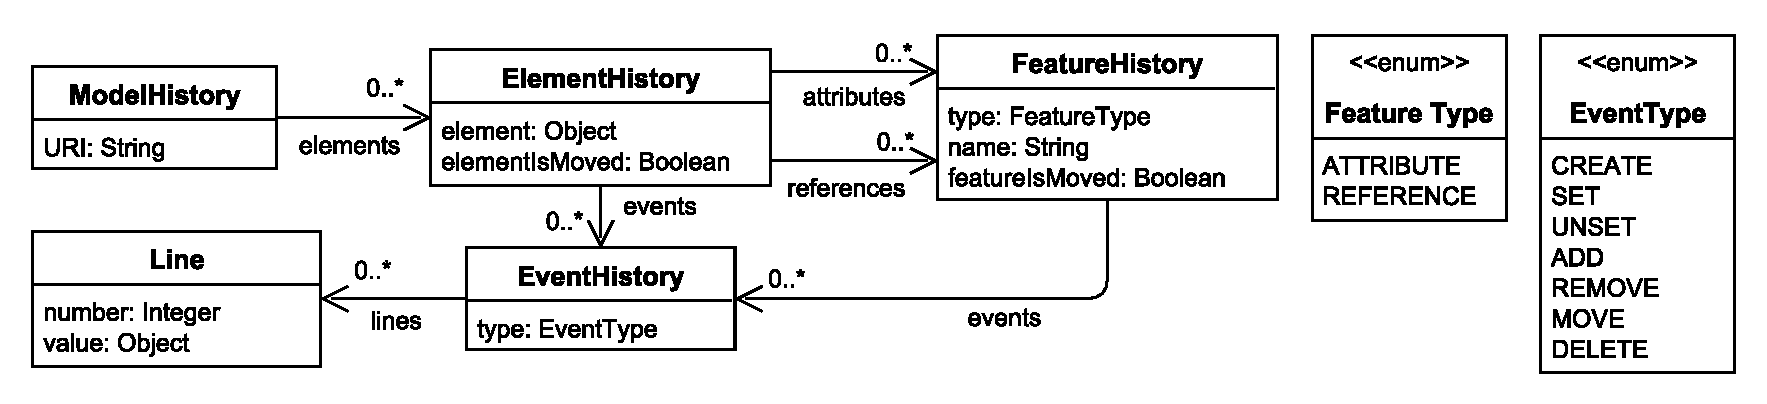
\includegraphics[width=\linewidth]{object_history}
%%	\caption{The class diagram of Model History.}
%%	\label{fig:object_history}
%%\end{figure}
%%
%%\begin{figure}[ht]
%%	\centering
%%	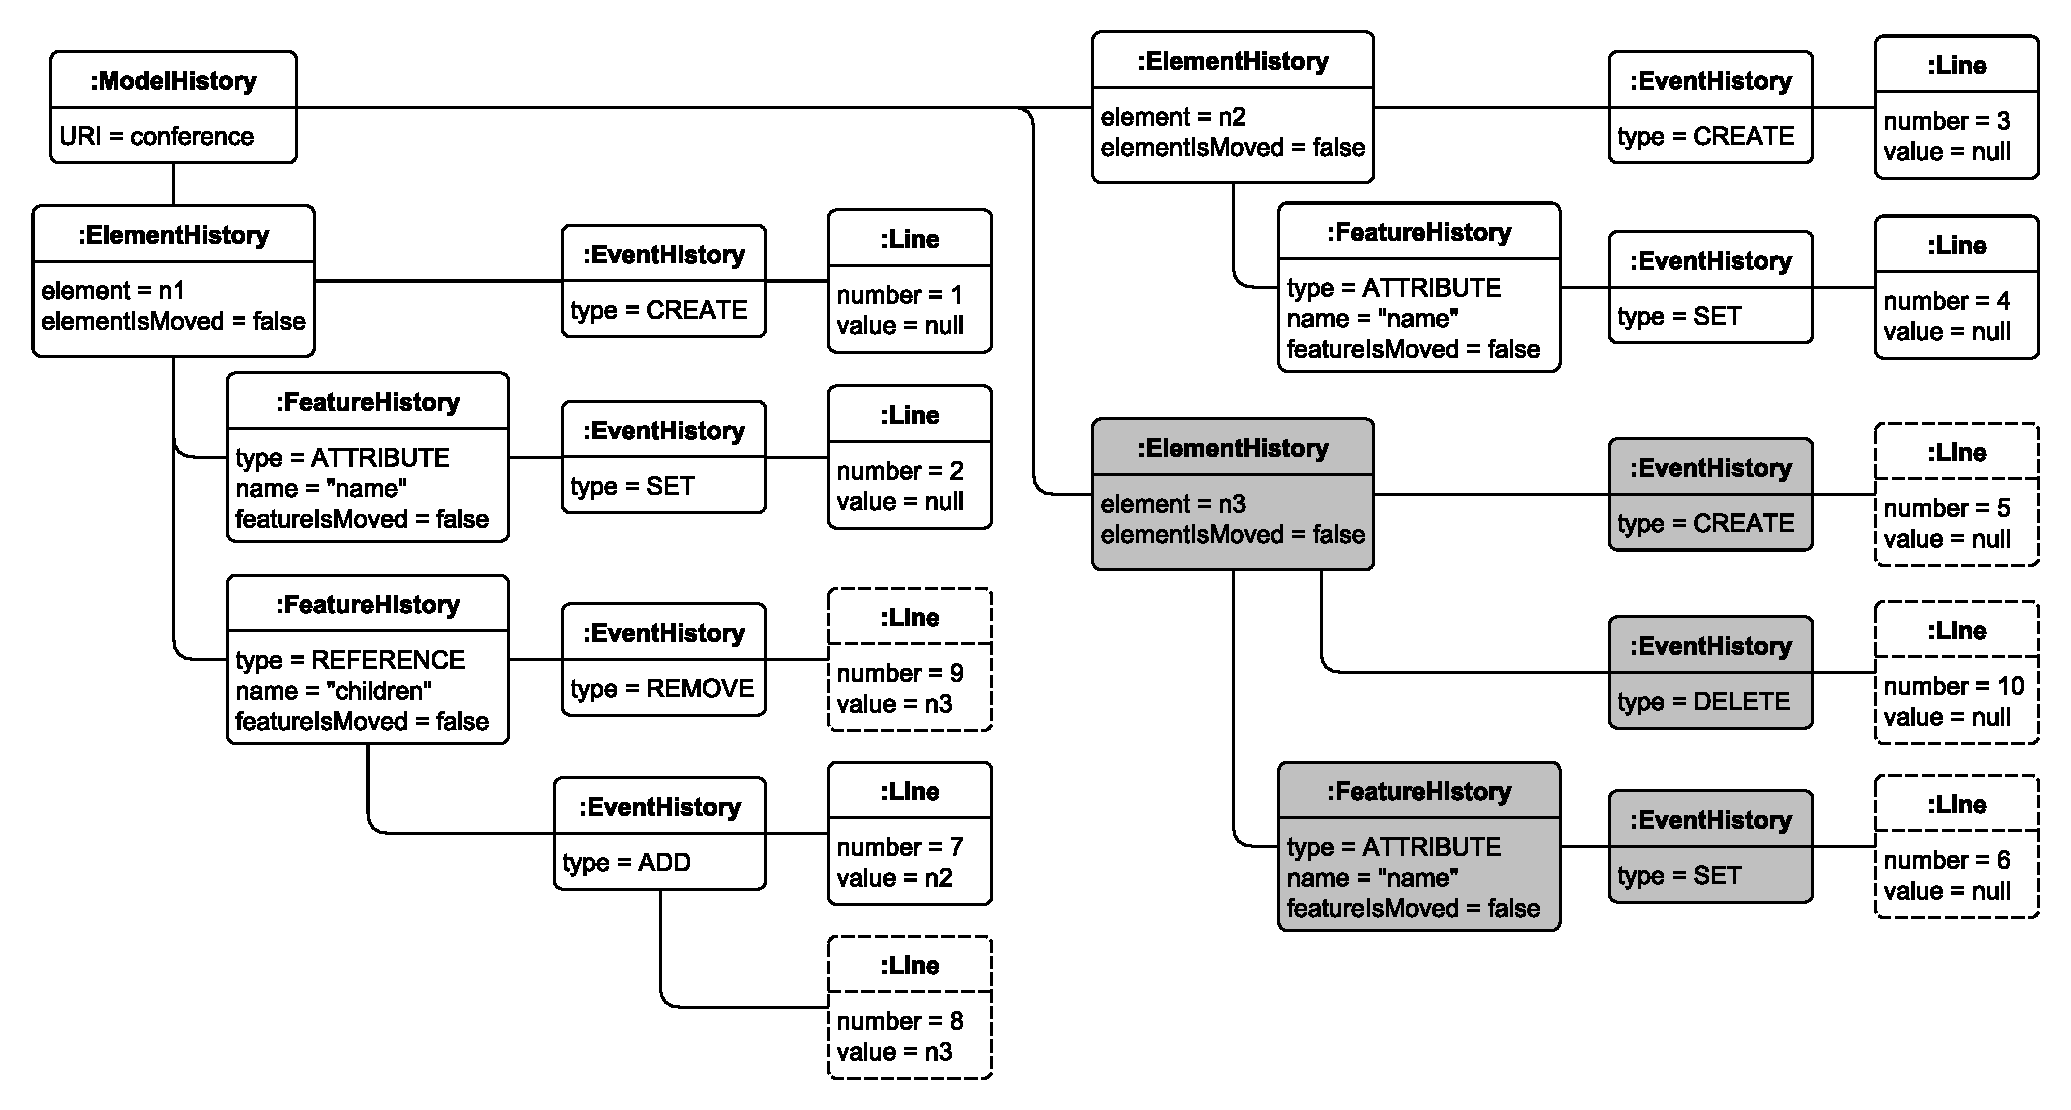
\includegraphics[width=\linewidth]{history_structure}
%%	\caption{The object diagram of the model history of the change-based model in Listing \ref{lst:change-based persistencemodel}.}
%%	\label{fig:history_structure}
%%\end{figure}
%%
%%A \emph{ModelHistory} has a \emph{URI} attribute to identify the model for which it records changes and can have many \emph{ElementHistory} elements. An \emph{ElementHistory} has an \emph{element} field that identifies the element that it refers to and an \emph{elementIsMoved} boolean flag. The  \emph{elementIsMoved} flag is used to indicate a \emph{move} event for the element (Sect. \ref{subsec:add_remove_and_move_operations} provides details of its use). Every \emph{ElementHistory} can have many \emph{FeatureHistories} to represent the editing histories of individual features (i.e. references/attributes) of the element.  A \emph{FeatureHistory} has three fields: \emph{type} to identify the feature's type (attribute or reference), \emph{name} to identify the feature's name, and \emph{featureIsMoved} that has the same role as attribute \emph{elementIsMoved} in \emph{ElementHistory}.
%%
%%An \emph{EventHistory} represents series of events of the same type in the change-based model. An \emph{EventHistory} has an attribute \emph{type} to identify the events' type and can have many \emph{Line}s. A \emph{Line} has a \emph{number} attribute to store the event number in the change-based model and a \emph{value} that is used to store the element involved in the event (it is only used for \emph{ADD}, \emph{REMOVE} and \emph{MOVE} events).
%%
%%Each \emph{FeatureHistory} can have many \emph{EventHistories} to represent the events that modify the value of the feature. Each \emph{ElementHistory} can have many \emph{EventHistories} to represent events that affect the state of the element (life-cycle and relations to multivalued features).
%%
%%Fig. \ref{fig:history_structure} shows the object diagram of the model history of the change-based model in Listing \ref{lst:change-based persistencemodel}. The grey rectangles are \emph{History} objects related to the deleted node \emph{n3}. The rectangles with the dashed outline are \emph{Line} objects that represent superseded changes. The next sections present the algorithms that use the information stored in the model history data structure to identify events that have no impact on the final state of the model, i.e. superseded events. The algorithms produce the ignore list that is used in the proposed change-based persistence loading algorithm.
%%
%%\subsection{Set and Unset Events}
%%\label{subsec:set_and_unset_events}
%%During the lifecycle of a model, a single-valued feature can be assigned many times. Each of the assignments is persisted as an event in the change-based model. However, only the last assigned value is necessary to obtain the current state of the feature.  That is, all events but the last can be ignored. For example, in Listing \ref{lst:set_unset_example}, the feature \emph{name} is assigned the ``A" value, nullified (unset), and finally assigned the ``B" value. That is, in the last state of the model: \emph{n1.name = ``B"}. As a result, the loading process could ignore all previous change events (lines 2 and 3) and only replay the last assignment event (line 4). 
%%
%%\begin{lstlisting}[style=eol,caption={The change-based persistence representation of attribute \emph{name} assignments.},label=lst:set_unset_example]
%%create n1 of Node
%%set n1.name to "A"
%%unset n1.name
%%set n1.name to "B"
%%\end{lstlisting}
%%
%%The algorithm that identifies superseded \emph{SET} and \emph{UNSET} events for a feature is presented in Alg. \ref{alg:set_unset_optimisation}. The algorithm has two inputs: a list of event numbers of \emph{SET} events and a list of event numbers of \emph{UNSET} events. The output of the algorithm is an \emph{ignoreList} that includes the event numbers that are superseded. The inputs lists can be trivially constructed from the model history data structure. For the \emph{name} feature in Listing \ref{lst:set_unset_example} these are: $setEventNumbers = \{2,4\}$ and $unsetEventNumbers = \{3\}$.
%%
%%\begin{algorithm}[H]
%%	\begin{small}
%%		\SetKwInOut{Input}{input}
%%		\SetKwInOut{Output}{output}
%%		\Input{two lists of Integer $setEventNumbers$}
%%		\Output{a list of Integer $ignoreList$}
%%		\SetKwBlock{Beginn}{beginn}{ende}
%%		\Begin{
%%			$setLastLine$ $\leftarrow$ getLastLine($setEventNumbers$)\;
%%			$unsetLastLine$ $\leftarrow$ getLastLine($unsetEventNumbers$)\;
%%			\uIf{$setLastLine > unsetLastLine$}{
%%				$ignoreList \leftarrow (setEventNumbers \cup unsetEventNumbers) \setminus \{setLastLine\} $\;
%%			}
%%			\ElseIf{$setLastLine < unsetLastLine$}{
%%				$ignoreList \leftarrow (setEventNumbers \cup unsetEventNumbers)$\;
%%			}
%%			\Return{$ignoreList$}\;
%%		}
%%	\end{small}
%%	\caption{Algorithm to identify event numbers of superseded \emph{set} and \emph{unset} events}
%%	\label{alg:set_unset_optimisation}
%%\end{algorithm}
%%
%%The \emph{ignoreList} is populated as follows.
%%In lines 2 and 3, the last event number of each input list is stored in \emph{setLastLine} and \emph{unsetLastLine} respectively. If $setLastLine > unsetLastLine$ (line 4) then $ignoreList = (setEventNumbers \cup unsetEventNumbers) \setminus  \{setLastLine\} $, i.e. all events except the last \emph{SET} event can be ignored. If $setLastLine < unsetLastLine$ (line 6) then $ignoreList = (setEventNumbers \cup unsetEventNumbers)$, i.e. all events can be ignored. For the \emph{name} feature in Listing \ref{lst:set_unset_example}, $ignoreList = \{2, 3\}$.
%%
%%\subsection{Add, Remove, and Move Events}\label{subsec:add_remove_and_move_operations}
%%Similarly, the contents of a multi-valued feature can be modified many times. If the same element is added and removed multiple times,  only that last event is necessary to determine if the element should appear in the values of the feature. For example, in Listing \ref{lst:add_remove_move_reference},  nodes \emph{n2} and \emph{n3} are added to the \emph{children} feature of \emph{n1} (lines 4-5), and then \emph{n3} is removed (line 6). That is, in the last state of the model: \emph{n1.children = [n2]}. As a result, the loading process could ignore the events that represent the \emph{ADD} and \emph{REMOVE} events of \emph{n3}. So far, the algorithm only supports unique features (i.e. features that do not allow duplicate values). An extension to support duplicate values is part of this research's future work. 
%%
%%\begin{lstlisting}[style=eol,caption={Example of change-based persistence representation of attribute \emph{values}'s add and remove operations.},label=lst:add_remove_move_reference]
%%create n1 of Node
%%create n2 of Node
%%create n3 of Node
%%add n2 to n1.children
%%add n3 to n1.children
%%remove n3 from n1.children
%%\end{lstlisting}
%%
%%The algorithm that identifies superseded \emph{ADD} and \emph{REMOVE} events for a feature is presented in Alg. \ref{alg:add_remove_move_optimisation}. The algorithm has four inputs: a list of Line objects of \emph{ADD} events, a list of Line objects of \emph{REMOVE} events, the element of interest and a flag that indicates a \emph{MOVE} event on the analysed feature.  The output of the algorithm is an \emph{ignoreList} that includes the event numbers that are superseded. The inputs lists can be easily constructed from the Model History data structure. For the \emph{children} feature in Listing \ref{lst:add_remove_move_reference} these are: $addEventLines=\{\{4,n2\},\{5,n3\}\}$, $removeEventLines=\{\{6,n3\}\}$, $moveEventLines=\emptyset$, $operandValue=n3$, and $featureIsMoved=\mathrm{False}$.
%%
%%\begin{algorithm}[H]
%%	\begin{small}
%%		\SetKwInOut{Input}{input}
%%		\SetKwInOut{Output}{output}
%%		\SetKwProg{Struct}{struct}{}{end}
%%		\Struct{Line}{
%%			Integer $eventNumber$;
%%			Anytype $value$;
%%		}
%%		\Input{two lists of Line $addEventLines$, $removeEventLines$, a variable of Anytype $operandValue$, a variable of Boolean $featureIsMoved$} % and $moveEventLines$, , an variable of Feature $feature$}
%%		\Output{a list of Integer $ignoreList$}
%%		\SetKwBlock{Beginn}{beginn}{ende}
%%		\Begin{
%%			\If{$featureIsMoved$ = false}{
%%				$filteredAddLines$ $\leftarrow$ filterByValue($addEventLines$, $operandValue$)\;
%%				$filteredRemoveLines$ $\leftarrow$ filterByValue($removeEventLines$, $operandValue$)\;
%%				$addLastLine$ $\leftarrow$ getLastLine($filteredAddLines$)\;
%%				$removeLastLine$ $\leftarrow$ getLastLine($filteredRemoveLines$)\;
%%				\uIf{$addLastLine > removeLastLine$}{
%%					$ignoreList \leftarrow (filteredAddLines.eventNumber \cup filteredRemoveLines.eventNumber \setminus \{addLastLine\} $\;
%%				}
%%				\ElseIf{$addLastLine < removeLastLine$}{
%%					$ignoreList \leftarrow (filteredAddLines.eventNumber \cup filteredRemoveLines.eventNumber$\;
%%				}
%%			}
%%			\Return{$ignoreList$}\;
%%		}
%%	\end{small}
%%	\caption{Algorithm to identify event numbers of superseded \emph{add}, \emph{remove}, and \emph{move} events.}
%%	\label{alg:add_remove_move_optimisation}
%%\end{algorithm}
%%
%%\noindent
%%\begin{minipage}[t]{0.48\linewidth}
%%	\begin{lstlisting}[style=eol,caption={The change-based persistence representation of reference \emph{children}'s move event.},label=lst:move_attribute_example]
%%	create p of Node
%%	create n1
%%	create n2
%%	create n3
%%	add n1 to p.children
%%	add n2 to p.children
%%	add n3 to p.children
%%	move from 0 to 1 in p.children
%%	remove n2 from p.children
%%	\end{lstlisting}
%%\end{minipage}
%%\hfill
%%\begin{minipage}[t]{0.48\linewidth}
%%	\begin{lstlisting}[style=eol,caption={The effective change-based persistence representation of reference \emph{children}'s move event.},label=lst:move_attribute_example_error]
%%	create p of Node
%%	create n1
%%	create n2
%%	create n3
%%	add n1 to p.children
%%	add n3 to p.children
%%	move from 0 to 1 in p.children
%%	\end{lstlisting}
%%\end{minipage}
%%
%%The \emph{ignoreList} is populated as follows. If the flag \emph{featureIsMoved} is true then nothing is added to the list (the need for this flag is explained later in this section). If the flag \emph{featureIsMoved} is false, then lines 6 and 7 filter the $addEventLines$ and $removeEventLines$ to only keep Lines for which the \emph{value} is equal to \emph{operandValue}. The filtered lists are stored in $filteredAddLines$ and $filteredRemoveLines$ respectively. The rest of the algorithm works similar to Alg. \ref{alg:set_unset_optimisation}, ignoring all events but the last if it was an \emph{ADD}, else ignoring all events. 
%%
%%The flag \emph{featureIsMoved} in line 5 in Alg. \ref{alg:add_remove_move_optimisation} is required to prevent ordering errors in the final state. As an illustration, the final states of the original change-based model presented in Listing  \ref{lst:move_attribute_example} and the effective change-based model of Listing \ref{lst:move_attribute_example_error} which \emph{does not} consider the \emph{featureIsMoved} flag are compared. In the effective change-based model, the events related to \emph{n2} have been ignored. Notice that the final state of the effective version is $p.values = [n3, n1]$  which is different from the original version $p.values = [n1, n3]$. The reason is that the move event in line 8 in the original version works on a different value than the one in the effective version.
%%
%%\subsection{Create and Delete Events}
%%\label{subsec:create_and_delete_operations}
%%When an element is deleted, it is completely removed from the model. Therefore, all events (create, set, unset, move, add, remove, delete) related to the element that happened before the event can be ignored, including all events related to its features, unless the element has been moved. For example, when node \emph{n3} in Listing \ref{lst:change-based persistencemodel}  is deleted, the events in lines 5-6 and 8-10 are superseded. The effective change-based model of Listing \ref{lst:change-based persistencemodel} is presented in Listing \ref{lst:change-based persistencemodel_optimised}.
%%
%%\begin{lstlisting}[style=eol,caption={Change-based representation of the model of Fig. \ref{fig:initial_model} after removal of node \emph{n5}.},label=lst:change-based persistencemodel_optimised]
%%create n1 of Node
%%set n1.name to "A"
%%create n2 of Node
%%set n2.name to "B"
%%add n2 to n1.children
%%\end{lstlisting}
%%
%%\begin{algorithm}[H]
%%    \begin{small}
%%        \SetKwInOut{Input}{input}
%%        \SetKwInOut{Output}{output}
%%        \Input{a variable of Object $deletedElement$, a list of Integer $ignoreList$}
%%        \Output{a list of Integer $ignoreList$}
%%        \Begin{
%%            $elementIsMoved$ $\leftarrow$ isElementMoved($deletedElement$)\;
%%            \If{$elementIsMoved$ = false}{
%%                $eventHistoryList$ $\leftarrow$ getAllEventHistories($deletedElement$)\; 
%%                \ForEach{$eventHistory$ in $EventHistoryList$}{
%%                    $lineList$ $\leftarrow$ getLines($eventHistory$)\;
%%                    Add all event numbers in $lineList$ into $ignoreList$\; 
%%                }
%%                $featureList$ $\leftarrow$ getAllAttributes($deletedElement$)\;
%%                \ForEach{$attribute$ in $featureList$}{
%%                    $eventHistoryList$ $\leftarrow$ getAllEventHistories($feature$)\;
%%                    \ForEach{$eventHistory$ in $EventHistoryList$}{
%%                        $lineList$ $\leftarrow$ getLines($eventHistory$)\;
%%                        Add all event numbers in $lineList$ into $ignoreList$\; 
%%                    }       
%%                }   
%%            }
%%            \Return{$ignoreList$}\;
%%        }
%%    \end{small}
%%    \caption{Algorithm to identify lines that are ignored after \emph{delete} events}
%%    \label{alg:create_delete_optimisation}
%%\end{algorithm}
%%
%%The algorithm that identifies superseded events for a deleted element is presented in Alg. \ref{alg:create_delete_optimisation}. The algorithm has one input: the deleted element. The output of the algorithm is an \emph{ignoreList} that includes the event numbers that are superseded. The inputs lists can be trivially constructed from the model history data structure.
%%
%%The algorithm starts by computing flag \emph{elementIsMoved} to determine whether the \emph{deletedElement} is already moved or not (line 2).
%%If it is false then it is safe to remove all lines that refer to the element (line 3) (the reason for using this flag was explained in section \ref{subsec:add_remove_and_move_operations}), otherwise, no action is taken. The algorithm then retrieves all event histories (\emph{eventHistoryList}) that refer to the element (line 4) and iterates through each event history (lines 5-8). For every event history (\emph{eventHistory} -- line 5), the algorithm retrieves its lines \emph{lineList} (line 6) and puts all their event numbers into the \emph{ignoreList} (line 7). After that, the algorithm continues to iterate through all its features and puts all lines' event numbers into the \emph{ignoreList} (lines 12-15). Finally, the algorithm returns the \emph{ignoreList} as its output.
%%
%%\subsection{Performance Evaluation}
%%\label{subsec:performance_evaluation}
%%This work has developed the proposed efficient loading algorithm on top of the original change-based persistence implementation from \cite{yohannis2017turning} and evaluated the algorithm's model loading performance, as well as its memory footprint and its impact on the time required to save changes made to change-based models. The evaluation was performed on Windows Server 2008 R2 64-bit with an Intel Xeon E5530 @2.40 GHz (2 processors) processor, 36 GB of memory, and the Java SE Runtime Environment (build 1.8.0\_66-b18).
%%
%%\begin{figure}[htbp]
%%	\centering
%%	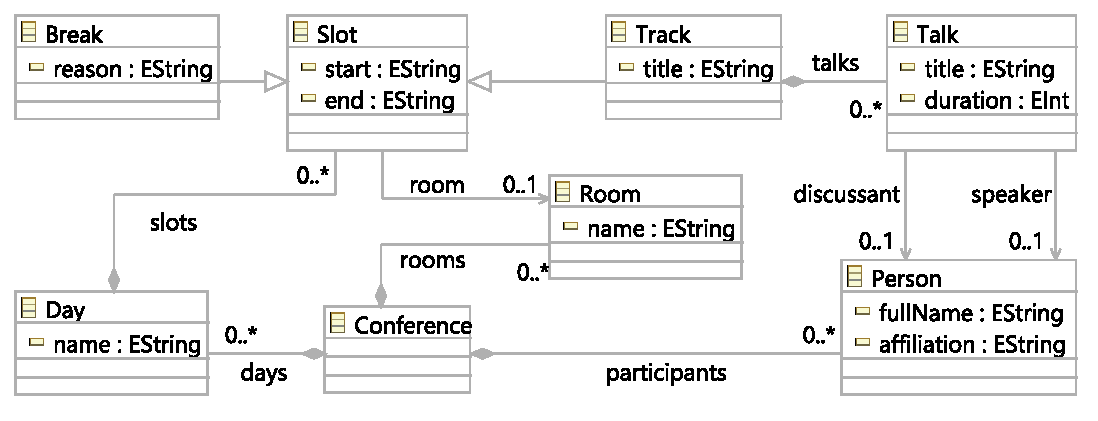
\includegraphics[width=0.9\linewidth]{conference_metamodel}
%%	\caption{The conference metamodel.}   
%%	\label{fig:node_metamodel}
%%\end{figure}
%%
%%For the evaluation experiments, this work has used synthetic models of different sizes conforming to the \emph{conference} metamodel in Fig. \ref{fig:node_metamodel}. This work has selected this metamodel as it provides reasonable coverage of the features of the EMF modelling capabilities such as single- and multi-valued features, inheritance, and containment and non-containment references. This work had little option other than to use synthetic models for the experiments given that change-based persistence is a very recent contribution and this work is not aware of any existing datasets containing real-world models expressed in a change-based format. Synthesising such models from existing state-based models (e.g. in XMI) was not an option either as state-based models do not capture editing-history-related information.    
%%
%%\subsubsection{Loading Time}
%%\label{subsec:loading_time_test}
%%
%%For this experiment, this work created and persisted change-based models of different sizes (from 500 up to 33,000 elements) conforming to the conference metamodel of Fig. \ref{fig:node_metamodel} through a random model generator that simulates the actions of a human modeller (i.e. creates/deletes elements, sets/unsets values of their features). This work then used the proposed and the baseline loading algorithms to reconstruct the state of these models and measured their execution time. The results are shown in Fig. \ref{fig:loading_speed_conf} and demonstrate the considerable time savings (up to 44\% faster compared to the original CPB implementation for the largest models) delivered by the proposed loading algorithm.
%%
%%\begin{figure}[ht]	
%%	\begin{subfigure}[t]{0.5\linewidth}
%%		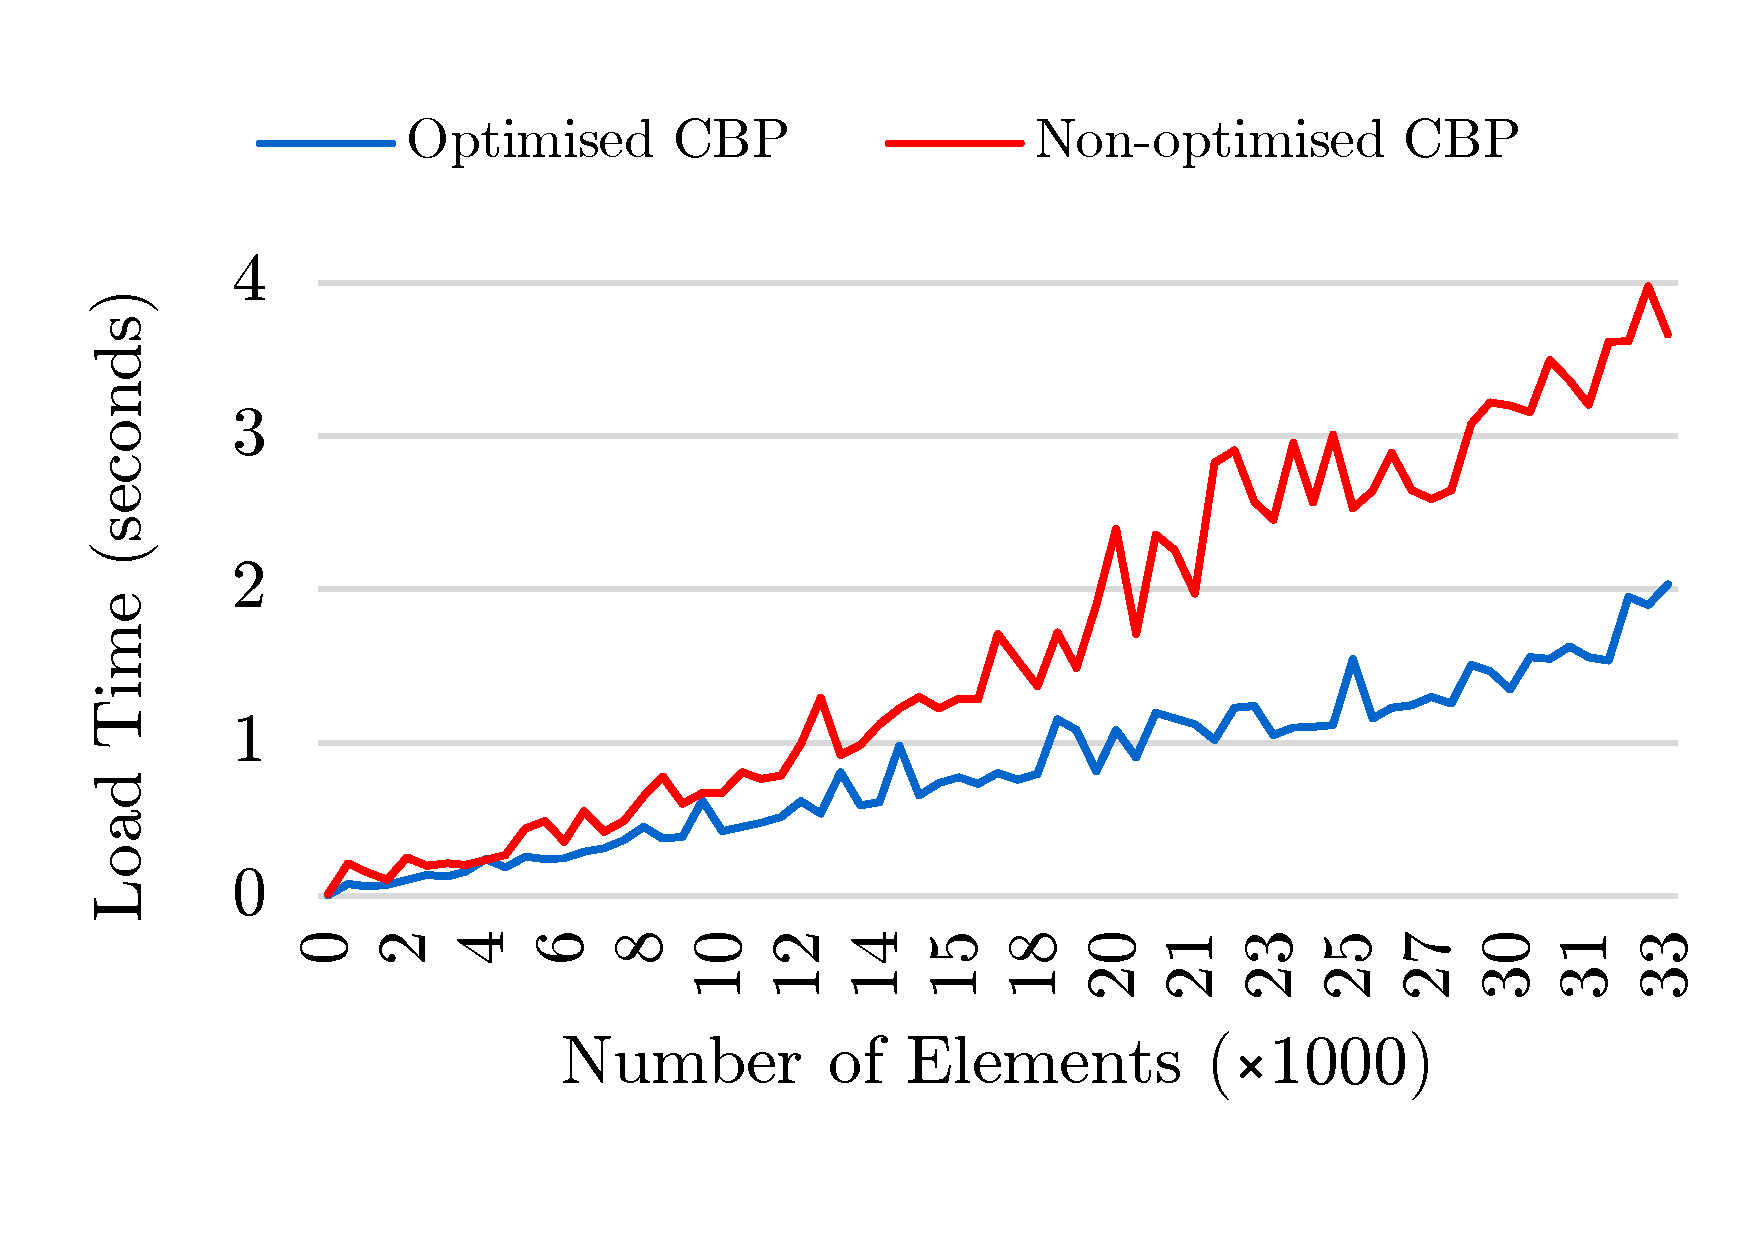
\includegraphics[width=\linewidth]{loading_speed_conf}
%%		\caption{Optimised change-based persistence vs Non-optimised change-based persistence}\label{fig:loading_speed_conf}
%%	\end{subfigure}
%%	\hfill
%%	\begin{subfigure}[t]{0.5\linewidth}
%%		\includegraphics[width=\linewidth]{loading_speed_conf_ochange-based persistence_xmi}
%%		\caption{Optimised change-based persistence vs XMI}\label{fig:loading_speed_conf_ochange-based persistence_xmi}		
%%	\end{subfigure}	
%%	\caption{A comparison on load time between optimised change-based persistence, non-optimised change-based persistence, and XMI.}
%%	\label{fig:loading_speed}
%%\end{figure}
%%
%%For reference, this work also contrasts the execution time for the proposed algorithm against that of loading the equivalent state-based model in XMI. As can be observed in Fig. \ref{fig:loading_speed_conf_ochange-based persistence_xmi}, despite the improvements delivered by the new algorithm, loading change-based models is still roughly 10 times slower than their state-based counterparts. However, as discussed in\,\cite{yohannis2017turning}, this can be an acceptable trade-off considering the other benefits that change-based model persistence has the potential to offer (e.g. more precise differencing and hence more efficient incremental execution of model management programs and more effective model merging).
%%
%%\subsubsection{Saving Time}
%%\label{subsec:saving_time_test}
%%
%%To achieve the benefits in terms of loading time demonstrated in Section \ref{subsec:loading_time_test}, the algorithm requires additional work to be done (i.e. to assemble the model history data structure and compute the ignore list delta) during the model saving phase as discussed in Section \ref{subsec:case_study}. To assess the impact of this additional work on the overall time required to save changes in models, this work used a random model generator to build up multiple versions of a conference model through random sequences of creating, deleting and modifying model elements, starting with an empty model and growing it up to 21,000 elements. Every 100 new elements, the generator would save the changes and measure the time required for this activity to complete. This work repeated the experiment with the prototype, with the existing baseline change-based persistence implementation and with state-based models stored in XMI.
%%
%%\begin{figure}[ht]	
%%	\begin{subfigure}[t]{0.5\linewidth}
%%		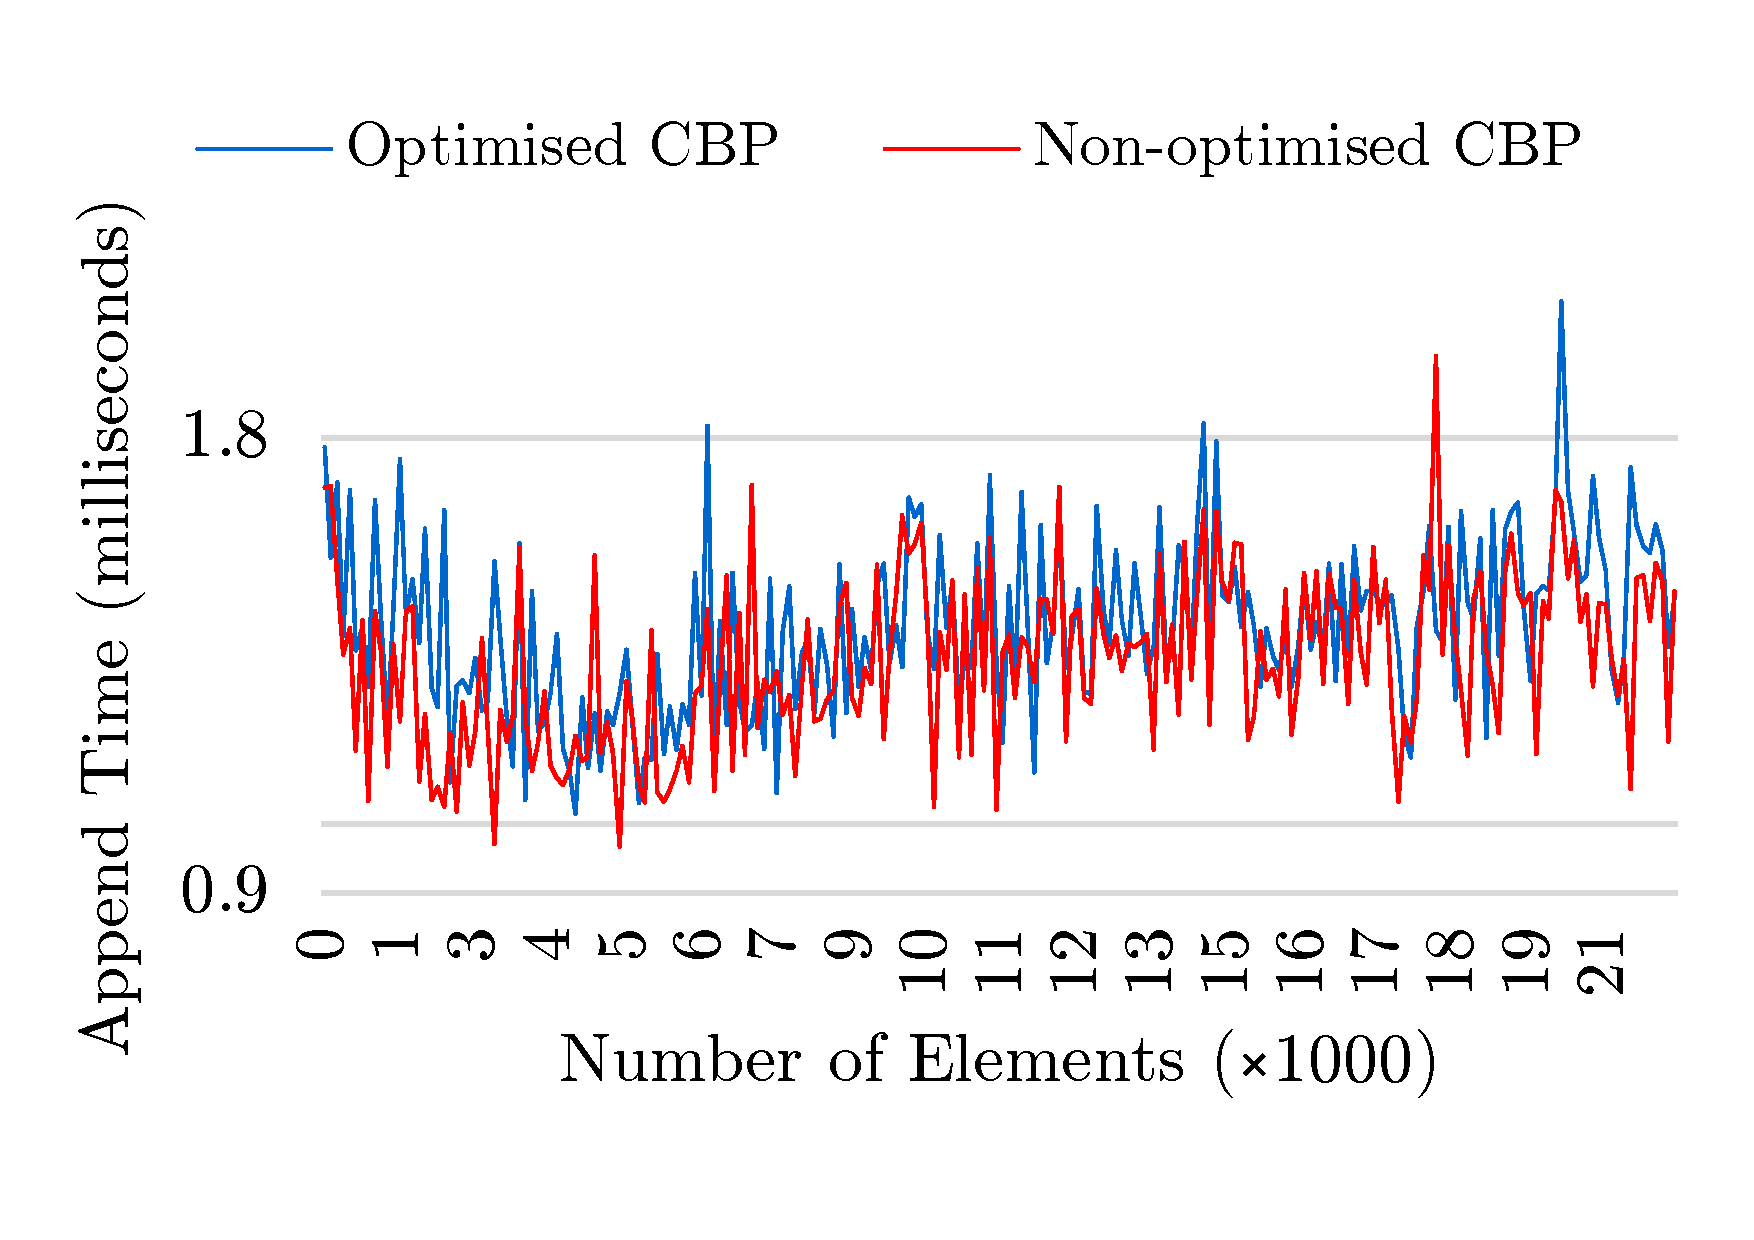
\includegraphics[width=\linewidth]{append_speed_conf}
%%		\caption{Optimised vs non-optimised change-based persistences}\label{fig:append_speed_conf}
%%	\end{subfigure}
%%	\hfill
%%	\begin{subfigure}[t]{0.5\linewidth}
%%		\includegraphics[width=\linewidth]{append_speed_conf_ochange-based persistence_xmi}
%%		\caption{Optimised change-based persistence vs XMI}\label{fig:append_speed_conf_ochange-based persistence_xmi}		
%%	\end{subfigure}	
%%	\caption{A comparison on time used to persist models between optimised change-based persistence, non-optimised change-based persistence, and XMI. The y-axis is $log_2$ scaled.}
%%	\label{fig:append_speed}
%%\end{figure}
%%
%%As shown in Fig. \ref{fig:append_speed_conf} the performance of the two change-based persistence implementations is almost indistinguishable, which indicates that the cost of the extra work needed by the proposed algorithm at this stage is negligible. On the other hand, change-based persistence implementations are significantly faster at saving changes than XMI. This is expected as the change-based persistence implementations only need to save the last set of changes every time by appending them to the existing model file (and hence their performance is relative to the number of changes since last saved), while the XMI implementation needs to reconstruct an XML document for the entire state of the model and replace the contents of the model file every time (and hence its performance is relative to the size of the entire model). 
%%
%%\subsubsection{Memory Footprint}
%%\label{subsec:memory_consumption}
%%As the proposed loading algorithm requires the maintenance of an additional in-memory data structure that keeps track of element and feature editing histories (see Fig. \ref{fig:history_structure}), This work conducted an additional experiment to measure its memory footprint. As with the experiment in Sect. \ref{subsec:saving_time_test}, this work used a random model generator to build up a conference model through random sequences of creating, deleting and modifying model elements, starting with an empty model and growing it up to 10,000 elements. Every 100 new elements, this work measured the memory consumed by the program. The results are plotted in Fig. \ref{fig:memory_ochange-based persistence_change-based persistence_xmi} and demonstrate the significant overhead of the used data structure.
%%
%%For reference, this work also includes the memory footprints of XMI in Fig. \ref{fig:memory_ochange-based persistence_change-based persistence_xmi} to contrast it with both change-based persistence implementations. As observed, XMI outperforms the optimised change-based persistence representation and performs slightly better than the original change-based persistence representation in terms of its memory footprint. 
%%
%%\begin{figure}[H]	
%%	\centering
%%	\includegraphics[width=\linewidth]{memory_ochange-based persistence_change-based persistence_xmi}
%%	\caption{A comparison on memory footprints between optimised change-based persistence, non-optimised change-based persistence, and XMI after loading models.}\label{fig:memory_ochange-based persistence_change-based persistence_xmi}
%%\end{figure}
%%
%%\subsubsection{Threats to Validity and Limitations}
%%\label{sec:limitations_and_future_work}
%%In this work, this work has only tested the algorithm on synthesised conference models which may not be representative of the complexity and interconnectedness of models in other domains. Diverse characteristics of models in different domains can affect the effectiveness of the algorithm and therefore yield different outcomes. 
%%
%%This work only supports ordered and unique features so far. Support for duplicate values means that removal of an item does not necessarily result in the item not being present in the feature value. Additional information must be captured to persist the number of copies and positions of the feature members. In the algorithms, this information can be used to generate the ignore list properly. In the case of unordered features, ``moved'' events do not exist, and hence further analysis is required to determine how this affects the use of the \emph{featureIsMoved} flag. 

\section{Evaluation Strategy}
\label{sec:evaluation_strategy}
For evaluations where there are existing approaches that the algorithms and tools developed in this research seek to outperform (e.g. change-based incremental validation vs state-based incremental validation), comparative evaluations will be conducted to assess the benefits and limitations of the approaches. For algorithms and tools that have no direct competitors in the literature, such as reducing file size and loading time of change-based models, their contributions will be assessed in comparison to the baseline they seek to improve (e.g. in this case, persisting and replaying full change histories).  

The evaluation strategy for each research question (Section \ref{sec:research_questions}) is as follows. 
\begin{enumerate}
    \item \textbf{Research Question 1.} The proposed change-based persistence will be evaluated for its correctness by comparing the eventual states of models persisted in change-based format to the same models persisted in state-based format. If they are equal, it means that the implementation has successfully loaded the change-based models. To perform the comparison, the process will start with an initial model -- empty or with several elements. Random operations (e.g. create, delete, add, remove, move, set, unset, etc.) then will be executed to modify the model. As the model grows, the models will be saved into a change-based file and a state-based file. After that, the change-based file will be loaded (replayed) to produce the eventual state of the model and then compared to the state-based file. The comparison will be performed iteratively at certain increment of number of elements (e.g. every increment of 500 elements). 
    
    The change-based persistence will also be compared to state-based persistence on their execution time and memory footprints of saving changes. The evaluation will use the same approach as above, except for saving the model into files, the saving will be performed every time a random operation executed. For the change-based persistence, only the changes that will be persisted, while for the state-based persistence, the entire model will be persisted.
    
    \item \textbf{Research Question 2.} The proposed solution to reduce the increasing file size of change-based models will be evaluated against the naive approach of saving change-based models. The comparison will be on their file size and memory footprints used to save models. For solution to reduce the loading time of change-based models by cancelling out preceded changes, the solution will be evaluated against the naive appraoch of loading change-based models by comparing them on on their loading time and memory footprints to load models. 
    
    For solution to reduce the loading time of models using change-based and state-based persistence side-by-side,  the hybrid approach will be evaluated on the time required to save changes, disk space usage, change-detection, and loading/query time. The hybrid approach will be compared against change-based persistence on time required to save changes and the disk space usage. The saving time and the disk space usage are selected as the dimensions of measurement since hybrid persistence will save changes into two kinds of persistence -- change-based persistence and state-based persistence -- which means it requires more saving time and disk space usage. The hybrid approach will also be compared against state-based persistence on time used for loading models since the intention of using the hybrid approach is to maintain the loading time of state-based persistence. 
    
    \item \textbf{Research Question 3.} This evaluation aims to understand to what extent detecting changes in change-based models performs against detecting changes in state-based models. The proposed solution will be compared to a state-based persistence implementation (e.g. EMF Compare) on the time and memory required to find all changes made to a model. Random operations (e.g. create, add, delete, remove, set, unset, move) will be executed programmatically to create a number of changes on the model and will be increased along iterations. 
    
    \item \textbf{Research Question 4.} This evaluation aims to understand to what extent comparison of change-based models performs against the comparison of state-based model. The proposed solution will be compared to a state-based persistence implementation (e.g. EMF Compare) on the time and memory required to find differences between two models that originate from the same ancestor. Random operations (e.g. create, add, delete, remove, set, unset, move) will be executed programmatically to create a number of differences between both models and will be increased along iterations. 
    
    \item \textbf{Research Question 5.} This evaluation aims to gain understanding to what extent change-based model merging performs against state-based model merging. The proposed solution will be compared to a state-based persistence implementation (e.g. EMF Compare) on the time and memory required to resolve conflicts and merge two different models that originate from the same ancestor. Some rules will be defined to resolve the conflicts programmatically and thus will remove the need for human intervention in the experiments; it is unlikely to ask a person to resolve many conflicts in large models. Random operations (e.g. create, add, delete, remove, set, unset, move) will be executed programmatically to create a number of differences between both models and will be increased along iterations. 
\end{enumerate}

\textbf{Model Datasets for Experiments.} Given that change-based persistence is a very recent contribution, and it is almost impossible to find any existing large model datasets containing real-world models expressed in change-based formats, this research will use synthetic models for experiments. Nevertheless, instead of synthesising the models arbitrarily, the change-based models will be obtained through reverse engineering. Several projects hosted on online version controls (e.g. GitHub) will be transformed using MoDisco\footnote{\url{https://www.eclipse.org/MoDisco/}} into models that confirm to Java metamodel\footnote{\url{https://help.eclipse.org/neon/index.jsp?topic=\%2Forg.eclipse.modisco.java.doc\%2Fmediawiki\%2Fjava_metamodel\%2Fuser.html}}. The differences between each version of the models are translated into change events in change-based models. Therefore, the generated change-based models are more representative since they are generated from real-world projects. The projects that will be selected are the projects that can generate large-scale Java models -- large-scale means a model consists of more than 1,500,000 elements as was experimented in NeoEMF \cite{daniel2016neoemf} and Morsa \cite{pagan2011morsa}. This strategy will be used in all tasks in the Research Plan (Section \ref{ch:research_plan}).

As an alternative for this method of model dataset generation, model datasets can also be produced by asking modellers to develop certain models using standard modelling languages such as UML and BPMN, and then persist the models in change-based format. The change-based models are then scaled-up to reach the criteria of 'large-scale' models. The drawback of such approach is that it depends on a number of modellers to generalise a pattern of developing certain models and it requires particular methods to identify the pattern.

\chapter{Research Plan}
\label{ch:research_plan}
For the next two years, this research plans to execute these following tasks. In every task, the correctness, performance, advantages, and shortcomings of the proposed change-based approaches are compared to equivalent approaches in state-based persistence. Every task, except Thesis Writing-Up, is expected to produce a publishable paper. The research timetable is displayed in Table \ref{table:research_timetable}.

\begin{table}[h]
    \centering
    \caption{Change-Based Persistence Research timetable.}
    \label{table:research_timetable}
    \begin{tabular}
        {|>{\centering\arraybackslash}p{1.1cm}|>{\centering\arraybackslash}p{4cm}|>{\centering\arraybackslash}p{4cm}|>{\centering\arraybackslash}p{4cm}|}
        \hline 
        Month & 2017 & 2018 & 2019 \\ 
        \hline 
        1               & \multirow{6}{4cm} & \multirow{3}{4cm}{\centering Hybrid Model Persistence}  & \multirow{2}{4cm}{\centering Task 5: File Size Reduction} \\ 
        \hhline{-~~~}2  & & &  \\ 
        \hhline{-~~-}3  & & & \textbf{40-Minute Seminar} \\ 
        \hhline{-~--}4  & & \textbf{Thesis Outline} & \multirow{5}{4cm}{\centering Task 6: Thesis Writing-Up}  \\ 
        \hhline{-~-~}5  & & \multirow{3}{4cm}{\centering Task 3: Model Change-Detection \& Comparison} & \\ 
        \hhline{-~~~}6  & & & \\ 
        \hhline{--~~}7  & \multirow{4}{4cm}{\centering Task 1: Change-Based Persistence \& Loading Optimisation} & &  \\  
        \hhline{-~-~}8  & & \textbf{Thesis Audit}  &  \\ 
        \hhline{-~--}9  & & \multirow{4}{4cm}{\centering Task 4: Model Merging} & \textbf{Thesis Submission} \\  
        \hhline{-~~-}10 & &  &  \\ 
        \hhline{--~~}11 & \textbf{Progress Report} &  &  \\ 
        \hhline{--~~}12 & \multirow{1}{4cm}{\centering Task 2:} & &  \\ 
        \hline 
    \end{tabular} 
\end{table}

\begin{itemize}
    \item \textbf{Task 1: Change-Based Persistence \& Loading Optimisation.}  The aim of this task is to prepare the ground for this research by developing a language-independent change-based model persistence format that can be used as a basis for hybrid model persistence, change-detection, model comparison, and model merging. Also, this task aims to design and implement an optimisation algorithm that reduces the loading time of change-based models by cancelling out events superseded by subsequent events. Five months was allocated for this task, and it already finished. Two papers had been written in this task. One paper was presented in a workshop, and another paper is under review. 
    \item \textbf{Task 2: Hybrid Model Persistence.} Based on the results of Task 1, this work found that although the proposed algorithm to optimise the loading time of change-based models can perform faster than loading the models naively, it is still outperformed by loading the same models in state-based persistence. Thus, this task will employ change-based and state-based persistence side-by-side to maintain the loading time of state-based persistence. Four months will be allocated for this task. Generating artificial models from existing version controls will be performed also is this task.  
    \item \textbf{Task 3: Model Change-Detection and Comparison.} This task will design and implement solution for detecting changes in change-based models and comparing change-based models with shared editing histories. Due to the nature of change-based models, it is expected that the solution developed in this task will differ substantially from current state-based model comparison algorithms. Three months will be allocated for this task. 
    \item \textbf{Task 4: Model Merging.} In this task, the candidate will design and implement solution for conflict resolution and merging of change-based models. The solution developed in this task will leverage/extend the comparison the solution developed in Task 3. Four months will be allocated for this task. 
    \item \textbf{Task 5: File Size Reduction.} This task will design and implement solution that can eliminate redundant changes within and across editing sessions, in order to reduce the storage requirements for persisting change-based models (e.g. if the value of a single-valued model element attribute is modified more than once in the context of an editing session, only the last modification event can be persisted). Since similar solution had already been applied to reduce the loading time of change-based models, the solution can also be applied to reduce the size of change-based files with some adjustments. Thus, only two months will be allocated for this task. It is important to notice that since the contribution of this task is relatively not as significant as other tasks, it will be given a lower priority than any other task and preferably to be dropped regarding limited time available.
    \item \textbf{Task 6: Thesis Writing-Up.} Five months will be allocated for the write-up of the doctoral thesis.  
\end{itemize}

\bibliographystyle{IEEEtran}
\bibliography{references}

\begin{appendices}
    \chapter{Publications}
    \label{ch:publications}
    Two papers have been written. The first paper \cite{yohannis2017turning} has been presented in the FlexMDE 2017 workshop and the second one \cite{yohannis2018algorithm} has been submitted to FASE 2018 and currently under review.
    \begin{enumerate}
        \item A. Yohannis, F. Polack, and D. Kolovos, ``Turning models inside out," in Proceedings of the 3rd Workshop on Flexible Model Driven Engineering co-located with ACM IEEE 20th International Conference on Model Driven Engineering Languages and Systems (MoDELS 2017), 2017.
        \item  A. Yohannis, H. Hoyos Rodriguez, F. Polack, and D. Kolovos, ``An algorithm for efficient loading of change-based models," submitted to the 21st International Conference on Fundamental Approaches to Software Engineering (FASE 2018) co-located with The European Joint Conferences on Theory and Practice of Software (ETAPS 2018), 2018 (under review).
    \end{enumerate}
\end{appendices}

%\begin{appendices}
%\end{appendices}

\end{document}